\chapter{Resultados}
\label{chap:resultados}

	\section{Projeção e visualização de APOO com Python}
	
	\subsection{Descrição da base}
	% TODO: descrever base de dados: quais foram os tipos de programas, quantos foram, falar que a
	% base foi anomizada.
		Essa base é constituída de 152 implementações de 5 problemas distintos. O primeiro exercício
		consiste na revisão de conceitos básicos como: estruturas de condição e laço de repetição. O
		segundo exercício define a criação de classes com mais de um construtor, e manipulação de
		arquivos e cadeia de caracteres. O terceiro exercício consiste na criação das classes
		\texttt{Palavra} e \texttt{Texto}, no qual a primeira classe deve ser utilizada na segunda
		classe, e uma classe para gerar orações gramaticais. O quarto exercício refere-se a
		utilização de herança e polimorfismo, identificando cada palavra contida em um arquivo. E
		o quinto exercício consiste na alteração de uma classe, implementando sobreposição de
		operadores. Os desenvolvedores das implementações foram anonimizados, sendo representado
		por uma sequência de números.
	
	\subsection{Avaliação da projeção com preservação de vizinhança}
	% TODO recomendo a colocação de uma imagem da curva de neihborhood  preservation para uma de suas projeções na seção resultados.
	A \foreign{Science View} (\cref{sec:scienceView}) utiliza a preservação da vizinhança
	(\cref{subsubsec:vizinhanca}) para verificar a qualidade das projeções. A \cref{fig:neighborhoodAPOO30}
	apresenta a qualidade da projeção para essa base de dados. O ponto de origem do
	gráfico condiz que não há perca de qualidade no eixo $x$, e não considera a quantidade
	de vizinhos no eixo $y$. Quanto maior o valor do eixo $x$, menor a qualidade da projeção.
	Quanto maior o valor do eixo $y$, maior a quantidade de vizinhos que está sendo analisado.
	
	Na \cref{fig:neighborhoodAPOO30} é possível observar que quanto menor a quantidade de
	instâncias a serem comparadas, menor a qualidade da projeção, como é possível observar
	nas curvas dos anos $1$ e $2$, nas cores vermelho e azul, respectivamente. Também é
	possível notar que a projeção perde 20\% de qualidade para as projeções dos anos
	$4$ e $5$ considerando a comparação de $30$ vizinhos do espaço $n$-dimensional com
	o espaço bidimensional.
	
	
	\begin{figure}
		\centering
		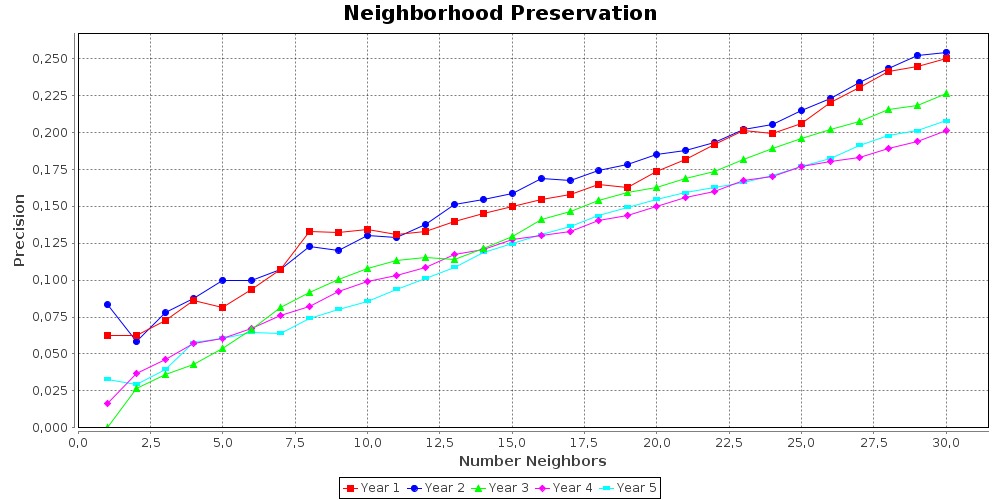
\includegraphics[width=0.7\linewidth]{imagem/neighborhoodAPOO30}
		\caption{Qualidade da projeção, utilizando a preservação de vizinhança (\foreign{neighborhood preservation})}
		\label{fig:neighborhoodAPOO30}
	\end{figure}
	
	
	\subsection{Avaliação qualitativa da visualização}
	% TODO: relatar o estudo: treinamento, instruções, questionário, resultados
		Para obter resultados qualitativos dessa pesquisa, realizamos um experimento com
		as seguintes etapas: treinamento, utilização e questionário. O treinamento foi
		realizado na forma de tutorial com a apresentação da ferramenta. Dessa forma,
		foi apresentado todos os passos para realizar uma nova projeção. Desde a inserção
		de uma nova coleção no banco de dados até a visualização das implementações. Em
		seguida, foi apresentado as funcionalidades da ferramenta para visualizar os
		agrupamentos formados ao longo das projeções, selecionar um determinado conjunto
		de implementações, identificar as características semelhantes de tais grupos e
		abrir mais de uma implementação simultaneamente.
		
		Para iniciarmos a etapa da utilização da ferramenta, foi pedido para que os
		participantes encerrassem o funcionamento da \foreign{Science View} e a
		executassem com a criação da base de dados. Os participantes utilizaram a
		ferramenta sem ajuda no que já tinha sido apresentado e o avaliaram por meio
		de um questionário.
		
		O questionário (\cref{apendice:questionario}) apresenta questões objetivas e
		dissertativas para avaliar a qualidade do treinamento e da ferramenta. Enquanto
		as questões objetivas visavam a qualidade do treinamento, da ferramenta e se
		é possível utilizá-la para auxiliar na correção, as questões dissertativas
		visam a encontrar lacunas observadas pelo participante para uma possível 
		atualização da ferramenta.
		
		A \cref{fig:projecaoFinal} apresenta a visualização dos agrupamentos das 152
		implementações contidas na base de dados. Isso foi possível após a adaptação da
		ferramenta para leitura de arquivos no formato \texttt{CSV}. Cada ponto da
		visualização é referente a um código-fonte. Ao clicar em um dos pontos, a
		\cref{fig:codigo1} mostra a exibição da sua implementação e as características
		extraídas das ferramentas para aquele código-fonte. Também é possível ordenar
		as colunas de características \foreign{Quantity} e \foreign{Normalized} em
		ordem  crescente ou decrescente para visualizar as características que mais
		ocorreram. Por padrão, a tabela é apresentado ordenada de forma descrescente
		pela coluna \foreign{Normalized}.
	
		\begin{figure}[h]
			\centering
			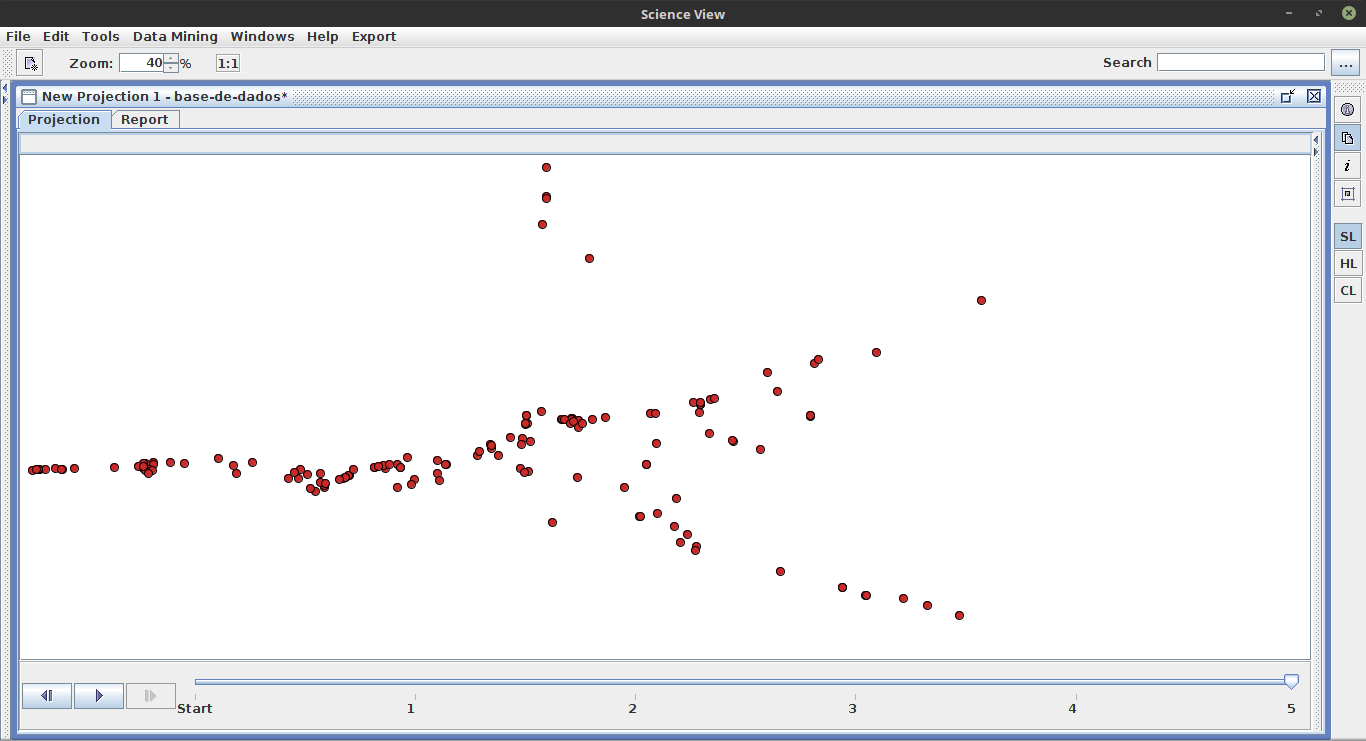
\includegraphics[width=1\linewidth]{imagem/projecaoFinal} % TODO: substituir, futuramente, pela figura da ferramenta corrigida.
			\caption[Visualização dos agrupamentos da base de dados gerado pela \texttt{Science View}]
			{Visualização dos agrupamentos da base de dados gerado pela \texttt{Science View} \cite{Alencar-etal:2012}}
			\label{fig:projecaoFinal}
		\end{figure}
		
		As implementações das \cref{fig:codigo1} e \cref{fig:codigo2} foram consideradas
		semelhantes, devido aos seus respectivos pontos estarem próximos no mapa de
		projeção. É possível notar que há diversas semelhanças nos tipos das características
		extraídas e erros que ocorreram pela coluna \foreign{Normalized}, além da quantidade
		dessas características apresentadas na coluna \foreign{Quantity}.
		
		\begin{figure}[h]
			\centering
			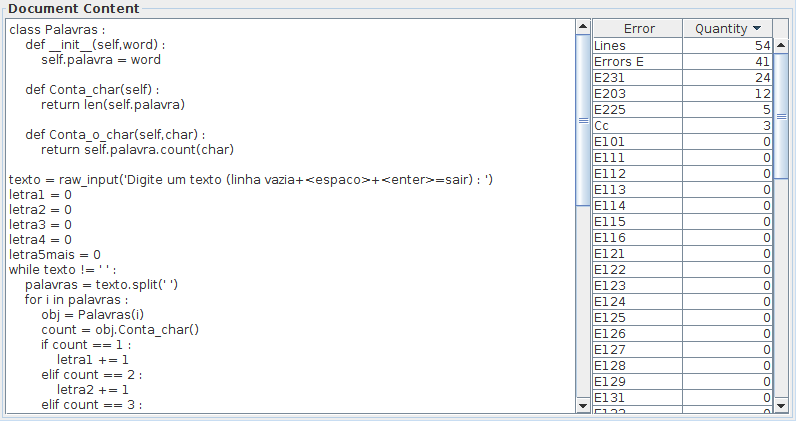
\includegraphics[width=0.8\linewidth]{imagem/codigo1}
			\caption[Representação parcial da interface que apresenta o código e suas características]
			{Representação parcial da interface que apresenta o código e suas características \cite{Alencar-etal:2012}}
			\label{fig:codigo1}
		\end{figure}
		
		\begin{figure}[H]
			\centering
			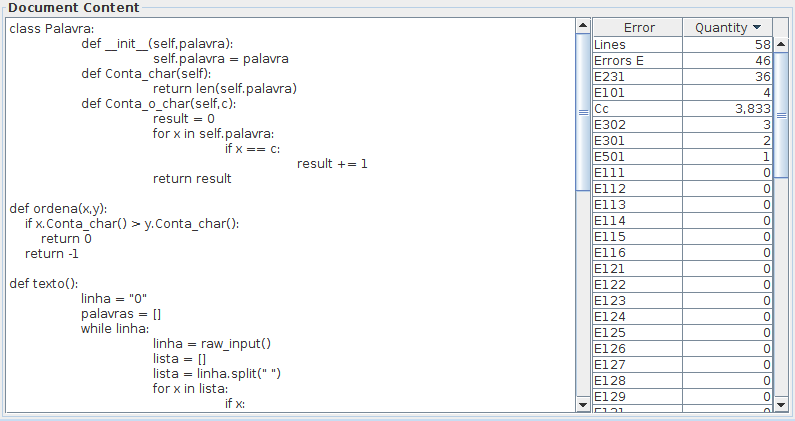
\includegraphics[width=0.8\linewidth]{imagem/codigo2}
			\caption[Representação parcial da interface que apresenta o código considerado semelhante ao da \cref{fig:codigo1}]
			{Representação parcial da interface que apresenta o código considerado semelhante ao da \cref{fig:codigo1} \cite{Alencar-etal:2012}}
			\label{fig:codigo2}
		\end{figure}
	
	
	\section{Projeção e visualização de MIT 6.00.1x}	

	\subsection{Descrição da base}
	% TODO: descrever base de dados: quais foram os tipos de programas, quantos foram, falar que a
	% base não foi anonimizada porque os programas estavam publicamente disponíveis no GitHub.
	Essa base de dados é constituída de 3470 implementações referente a 10 exercícios
	distintos. Todos as atividades solicitam manipulação de arquivo e cadeia de caracteres.
	
	O primeiro exercício requer conceitos de matriz, utilizando lista dentro
	de lista, e programação dinâmica para solucionar o transporte de animais.
	
	O segundo exercício necessita de conhecimento sobre aleatoriedade, lista, condicional,
	cadeia de caracteres, operações aritméticas e lógicas para implementar o jogo da
	forca.
	
	O terceiro exercício solicita a utilização de laço de repetição, condicional, lista,
	operações aritméticas e lógicas para implementar o jogo das palavras.
	
	O quarto exercício requer conhecimento de lista e dicionário pra codificar e
	decodificar um texto.
	O quinto exercício requer o uso de analisador (\foreign{parser}), construção
	de classe, interface, polimorfismo e operadores lógicos para desenvolver um programa
	de monitoramento de novos \foreign{feeds} na Internet.
	
	O sexto exercício solicita conhecimento sobre criação de classes, matriz, laço de
	repetição e manipulação de interface gráfica para implementar um aspirador de pó
	inteligente e sua simulação.
	
	O sétimo exercício consiste no uso de classes, aleatoriedade, laço de repetição,
	condicional, lista e conhecimento de estatística para implementar uma simulação
	e um sistema de tratamento de pacientes conforme o vírus que eles possuem.
	
	O oitavo problema consiste na implementação de classes a partir do exercício $7$.
	Pedindo a implementação da classe \texttt{ResistantVirus} e \texttt{SimplePatient}
	para realizar simulações desses vírus em pacientes.
	
	O nono exercício requer o uso de dicionário e operador lógico para desenvolver
	um software que apresente uma lista de assuntos para cada aluno da universidade.
	
	E para o décimo exercício, é necessário conhecer um algoritmo de agrupamento para
	realizar sua implementação.
	
	Os desenvolvedores dessas implementações não foram anonimizados, pois seus
	códigos-fontes estavam presentes em repositórios públicos no GitHub \cite{github}.
	
	% TODO: Marco: colocar a string utilizada para buscar os programas e como foi criada a base
	

\subsection{Avaliação da projeção com preservação de vizinhança}


\subsection{Avaliação qualitativa da visualização}
% TODO: relatar o estudo: treinamento, instruções, questionário, resultados



	\section{Considerações finais}
	
		O atual banco de dados de implementações, formado por 152 códigos-fontes que
		solucionam 5 problemas distintos é considerado pequeno e pode enviesar o
		projeto. Para isso, construiremos outro banco de dados de implementações
		por meio de submissões de voluntários, visando possuir um conjunto de
		implementações vasto para a pesquisa.
